\subsection{Methodological considerations}

In order to estimate the empirical variance of the estimators similarly to a Monte Carlo study, $100$ artificial samples of size $N \times m$ were created with the help of stratified sampling without replacement. \textcite{bickel2008choice} refer to this approach as the $m$-bootstrap, where $m$ refers to the block size or the percentage of data points from the original sample to be used to construct the new sample. Stratified subsampling works such that each time, random data points are taken only once from the full sample in order to create a subsample of smaller size while maintaining the original proportions of cases and controls. \\

The main practical problem while constructing the artificial samples is the choice of the block size \textit{m} (\cite{politis1999subsampling}). The selection of this block size is crucial since a size that is too small could hinder the subsampling estimates by further reducing their effective subsampling size. To ensure accuracy, I tested different values of block size $m=\{0.95, 0.9, 0.85, \dots, 0.45, 0.4\}$. In this way, for each value of $m$, a set of $100$ independent artificial samples was created. \\

An LCC pass was fitted to each data in a sample set, and its average subsample size was then used to obtain the LCC's fixed $N_s$, as in the Simulation section. However, a key difference here is that the effective subsample size for CC and WCC was not enough to ensure that they would have roughly twice as many data points as LCC. Thus, their acceptance probability was set such that $a(1)=1$ and $a(0) = (P(Y=1)a(1))/P(Y=0)$; in other words, it was necessary to subsample all cases and the same amount of controls. This approach was still not enough to provide a CC and WCC subsample size twice as large as the one for LCC, but it did help to approximate their desired dimension (see Appendix Section \ref{app:data-tables} for the exact fixes $N_s$ used in the analysis). The algorithms were then fitted to each artificial sample, thus obtaining $100$ realizations of each subsampling scheme and $m$ value. The variance of the estimates was calculated as outlined in Section \ref{sec:metrics}. 


\subsection{Results}

The results for the empirical variance of the estimates are shown in Table \ref{tab:data-res}. The block size $m=0.85$ shows the lowest empirical variances for all methods, and thus it is chosen as a robust block size for the analysis. 
Recall that this dataset refers to a scenario of large $N$, small $k$, mild-to-large marginal imbalance, and what appears to suggest low conditional imbalance. In this regard, we could expect that the results resemble the findings presented in panels 1 and 2 from Table\ref{tab:sim_prob_a2} of Section \ref{sec:sim3}, where it was shown that for mild marginal imbalance levels, CC, WCC, and LCC
perform similar in terms of variance.


% latex table generated in R 4.2.1 by xtable 1.8-4 package
% Sun Jun 11 13:26:25 2023
\begin{table}[ht]
\centering
\begin{tabular}{ccccc}
  \hline
$m$ & $\widehat{var}_{logit}$ & $\widehat{var}_{CC}$ & $\widehat{var}_{WCC}$ & $\widehat{var}_{LCC}$ \\ 
  \hline
0.95 & 0.0004 & 0.0071 & 0.0084 & 0.0077 \\ 
  0.90 & 0.0009 & 0.0100 & 0.0117 & 0.0084 \\ 
  %\rowcolor{yellow!30}
  0.85 & 0.0014 & 0.0097 & 0.0106 & 0.0084 \\ 
  0.80 & 0.0027 & 0.0114 & 0.0136 & 0.0103 \\ 
  0.75 & 0.0026 & 0.0110 & 0.0131 & 0.0125 \\ 
  0.70 & 0.0034 & 0.0127 & 0.0150 & 0.0148 \\ 
  0.65 & 0.0057 & 0.0121 & 0.0129 & 0.0200 \\ 
  0.60 & 0.0062 & 0.0195 & 0.0230 & 0.0161 \\ 
  0.55 & 0.0085 & 0.0197 & 0.0232 & 0.0207 \\ 
  0.50 & 0.0089 & 0.0267 & 0.0320 & 0.0304 \\ 
  0.45 & 0.0119 & 0.0337 & 0.0373 & 0.0305 \\ 
  0.40 & 0.0125 & 0.0301 & 0.0349 & 0.0294 \\ 
   \hline
\end{tabular}
\caption[Data application - Empirical variance results for the Income dataset]{Results for the Income dataset - Empirical variance of the $\hat{\theta}$ estimates for the three subsampling methods under different levels of subsampling $m$ for creating the synthetic samples.}
\label{tab:data-res}
\end{table}


As expected, the results for the Income dataset seem to agree with both the theory of the methods and the results from the numerical exercises. For $m=0.85$, LCC shows the lowest empirical variance among all case-control methods. However, unlike scenarios with high conditional imbalance, LCC does not fully dominate the other methods in terms of efficiency. In fact, its performance is not very different from the CC algorithm, which is not surprising given that CC has shown to perform well under high marginal imbalance. On the other hand, despite having the worst variance performance, WCC does not show to be underperforming so severely, mostly because the variation in the weights is not severe when the imbalance is mild. \\

Moreover, the LCC estimate displays an empirical variance $6$ times higher than the empirical variance of the logistic regression on the full sample. One explanation could be that the effective sample size for the LCC and its pilot is too small to approximate an asymptotic behavior ($N_s = 11,242$, see Appendix). However, in Simulation \ref{sec:sim2}, LCC had access to a much smaller sample size, and yet the estimate showed to be very close to its asymptotic behavior. Thus, it seems more likely that the loss in efficiency is primarily driven by the data dependency of the pilot and the low presence of conditional imbalance. \\

\begin{figure}[ht]
    \centering
    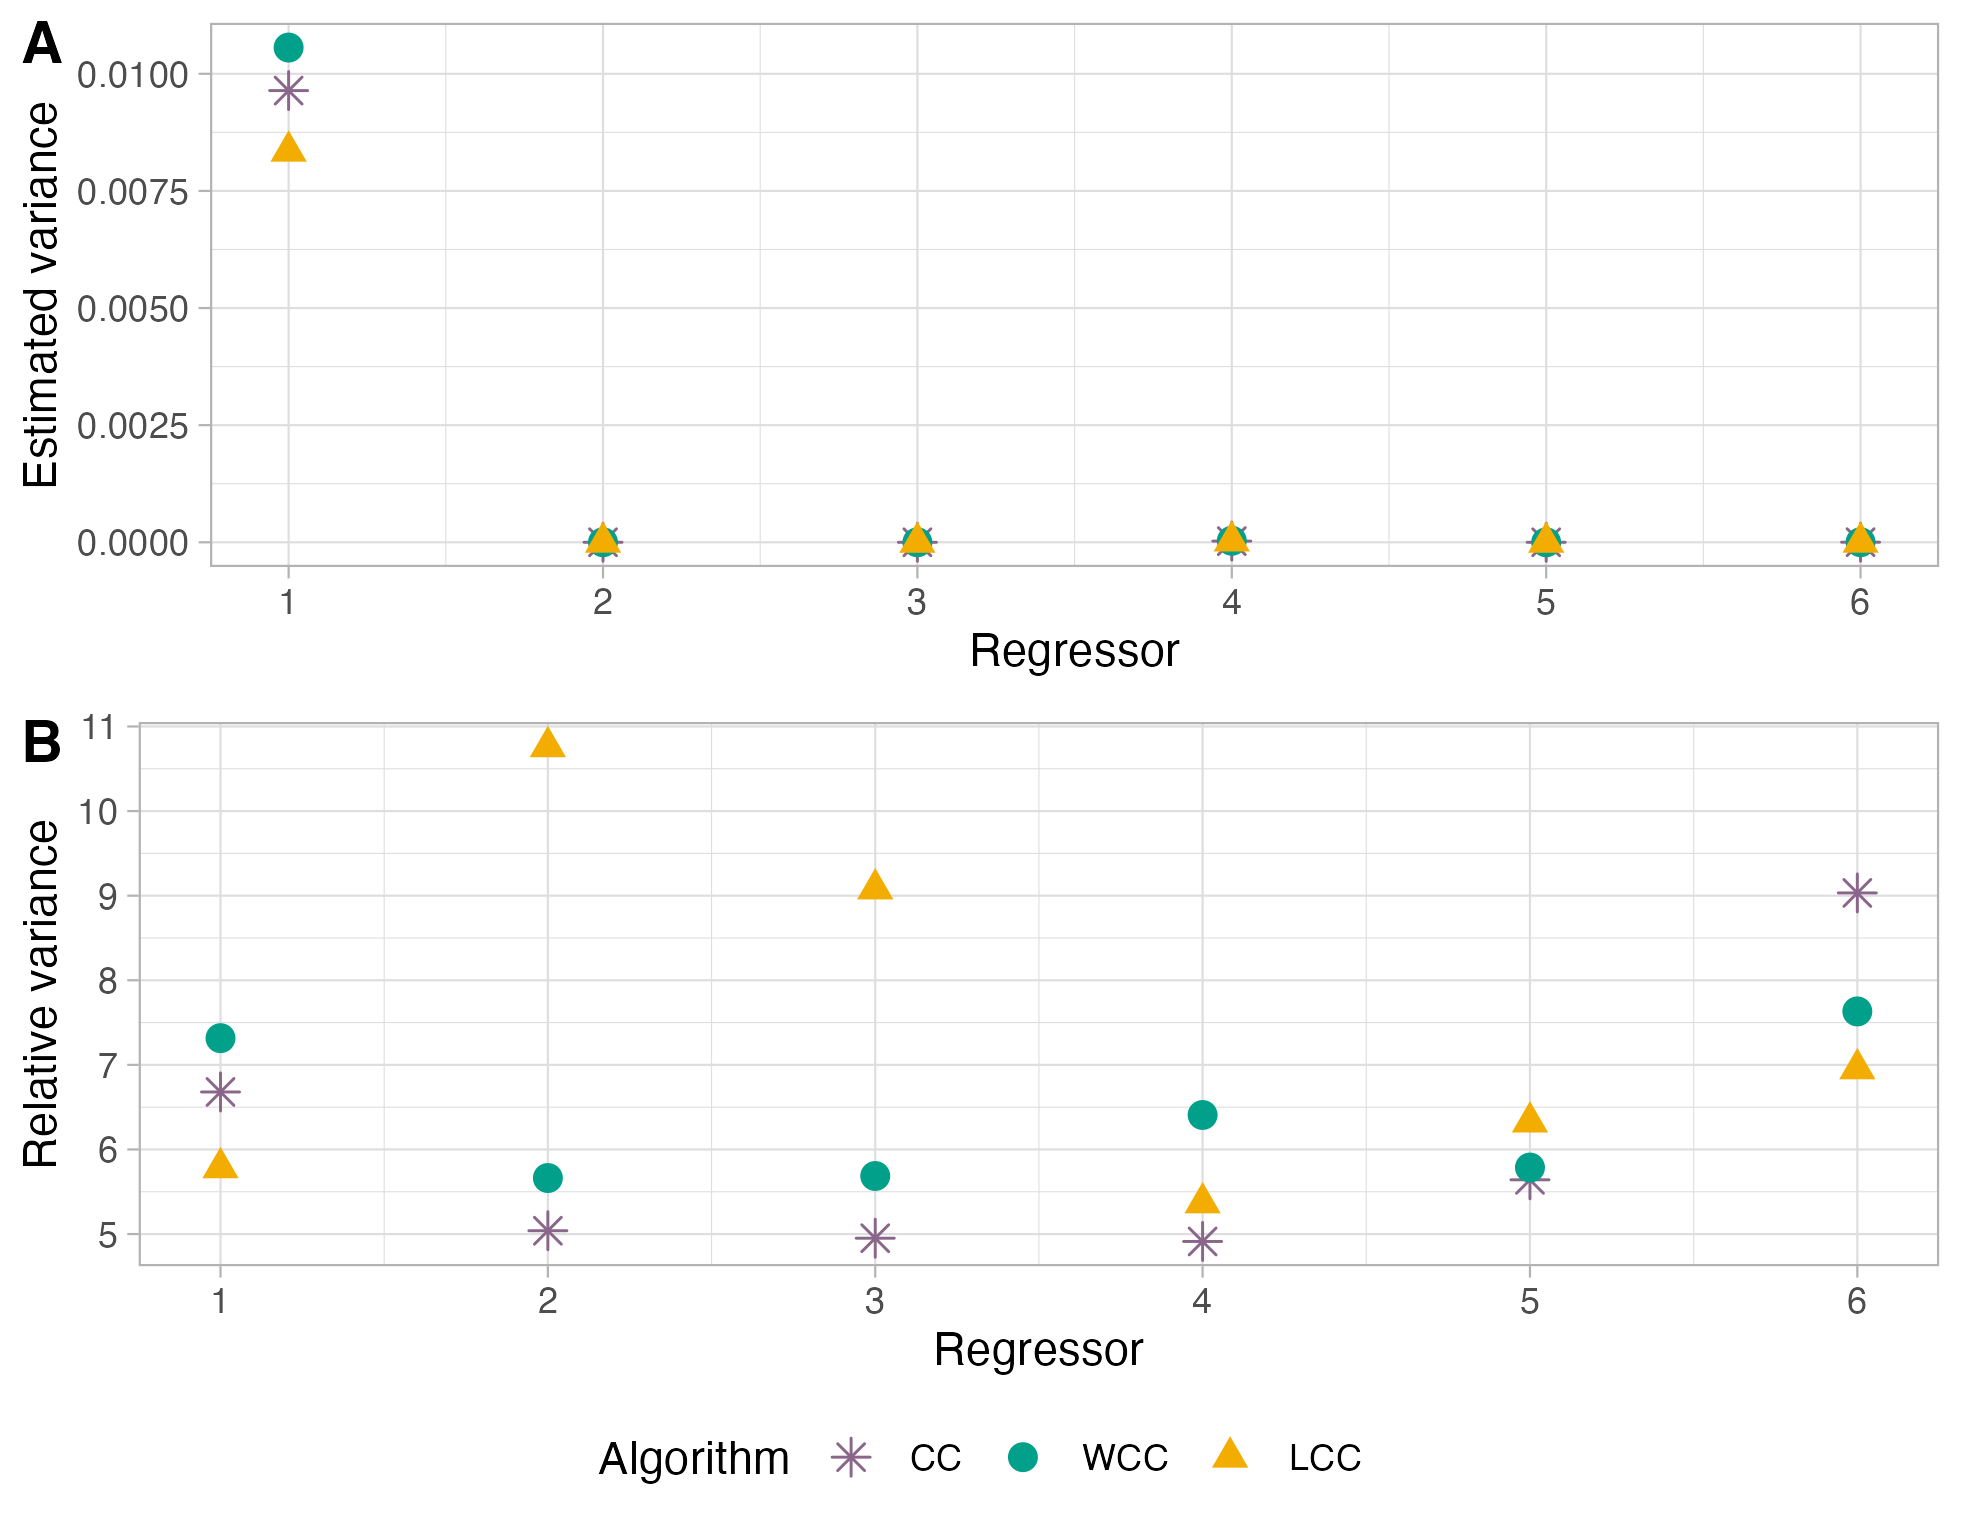
\includegraphics[scale=0.7]{2_Figures/all_variances.png}
    \caption[Data application - Relative variance of coefficients]{Empirical variance of coefficients, where: 1=intercept, 2=age, 3=fnlwgt, 4=years of education, 5=capital loss, and 6=hours per week. \textbf{Panel A.} Variance ratio of coefficients for the 3 different subsampling algorithms relative to full sample logistic regression variance. \textbf{Panel B.} Variance of coefficients for the 3 different subsampling algorithms.}
    \label{fig:all-vars-data}
\end{figure}

Figure \ref{fig:all-vars-data} Panel A shows the empirical variance of the coefficients by algorithm. The intercept term shows the largest variance of all, with LCC's coefficient displaying the lowest. For the other regressors, the variances are small and similar across methods. However, Panel B further decomposes the analysis and shows the variance of each coefficient relative to the variance of the full sample logistic regression. LCC shows the lowest ratio against the logistic regression estimate for the intercept but exhibits the largest relative variance for two slope coefficients, even reaching a ratio of $11$ times the full sample logistic regression for age's estimated coefficient. Overall, the analysis of the individual variance suggests that some of the LCC estimates have large individual noise, potentially caused by the utilization of a data-dependent pilot with its own variance, which may be impacting the general efficiency of LCC. Additionally, it is worth noting that logistic regression yields the most efficient coefficient among all methods and it is clear that, given the characteristics of the dataset, the trade-off between efficiency and computational gains is too costly. 

